\documentclass[10pt,letterpaper]{article}
\usepackage[margin=0.7in]{geometry}
\usepackage[T1]{fontenc}
\usepackage[utf8]{inputenc}
\usepackage{array,booktabs,tabularx,graphicx,placeins,amsmath,amssymb,url,cite}
\usepackage{hyperref,needspace}
\hypersetup{colorlinks=true,linkcolor=blue,citecolor=blue,urlcolor=blue}
\setlength{\parindent}{0pt}
\setlength{\parskip}{5pt}
\renewcommand{\thetable}{S\arabic{table}}
\renewcommand{\thefigure}{S\arabic{figure}}
\title{O-ISAC: Supplementary Evidence Profiles}
\author{Fatih D\"onmez, Ahmet Altuncu, and Mustafa Namdar}
\date{16 September 2026}
\begin{document}
\maketitle
These profiles accompany the systematic review of 206 studies represented by
227 eligible reports. They describe the distribution and interpretation of
the extracted evidence. The separate supplementary methods narrative documents
search, selection, extraction, synthesis, appraisal and limitations. The
source index links these materials to the complete study register and frozen
evidence tables in the review archive: \url{https://osf.io/7f6wb/}.

% Supplement fragment. Compile from the supplement/ directory.
\section{S-Core: Platform, Metric, and Relationship Evidence Profiles}
\label{supp:core}

\subsection{Platform Assignment}

The main-text platform table retains the canonical mutually exclusive family
counts for 206 studies. Each study is assigned to its dominant physical
platform, while physical media and integration mechanisms can overlap within
the same system. Transmitters supplied through fiber enter the photonic
terahertz family when photonic generation and conversion create the wireless
carrier directed at the target. Fiber remains the organizing platform when it
transports signals to downstream RFID, radio, or radar sensing. Hybrid
membership requires interaction across segments to shape the result. Family
counts describe corpus coverage rather than relative performance or maturity.

\subsection{Metric Evidence}

The primary synthesis contains 4,779 metric records. A record is an extraction
unit preserving a reported quantity, its available definition, conditions, and
source location; it is not an independent study or effect estimate. Data rate,
BER, and range resolution appear in 85, 60, and 50 studies, respectively, with
overlapping study coverage.

\begin{table}[htbp]
\caption{Domain coverage of the primary metric records}
\label{tab:s_metric_domains}
\centering
\footnotesize
\setlength{\tabcolsep}{4pt}
\begin{tabular}{@{}lrr@{}}
\toprule
Domain & Records, $n$ (\%) & Studies, $n$ (\%) \\
\midrule
Sensing & 1,816 (38.0\%) & 203 (98.5\%) \\
Communication & 1,328 (27.8\%) & 194 (94.2\%) \\
Joint & 870 (18.2\%) & 158 (76.7\%) \\
Implementation & 476 (10.0\%) & 64 (31.1\%) \\
Smaller normalized domains & 289 (6.0\%) & 33 (16.0\%) \\
\bottomrule
\end{tabular}
\end{table}

Domain rows partition the primary metric records, whereas study counts overlap.
Of these records, 118 (2.5\%) are conditional comparison candidates and 4,661
(97.5\%) retain their native-context analytical role. Candidate status requires
the reported definition, task, measurement plane, operating conditions, and
validation to be checked before any proposed comparison. It does not establish
a verified comparison across independent studies or justify pooling. The
remaining records support mechanism, feasibility, and qualitative synthesis in
their source contexts. The complete metric register contains 4,861 rows,
including 31 contextual records and 51 records documenting source conflicts.
Electronic Supplement S-Evidence preserves the complete records and provenance.

\subsection{Joint Performance Relationships}

The relationship register contains 404 entries. Two document the absence of a
tradeoff, leaving 402 substantive relationships from 168 studies. These include
218 quantitative and 184 qualitative records; 371 substantive relationships
have condition-dependent interpretations. The profile in
Fig.~\ref{fig:s_tradeoff_profile} preserves the overlapping mechanism-family
coverage. A relationship is not a study, a pooled effect, or an independently
verified cross-study comparison. The main text uses selected within-study
examples to explain how a shared choice changes communication and sensing.

\begin{figure*}[t]
\centering
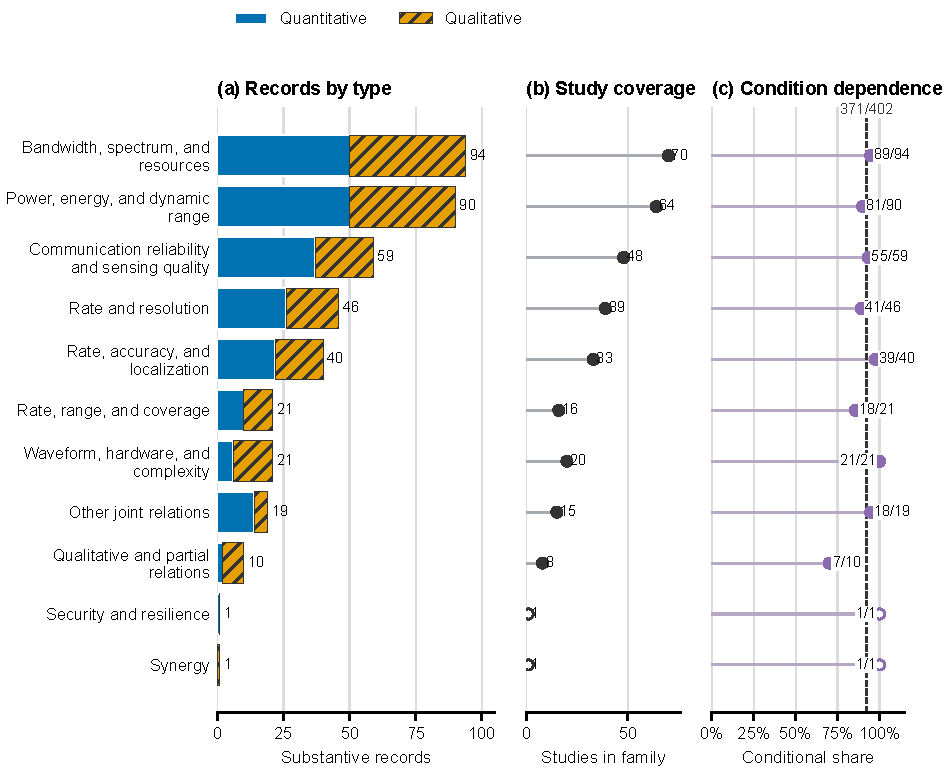
\includegraphics[width=\textwidth]{../manuscript/figures/final_submission_2026-08-25/fig06_tradeoff_profile.pdf}
\caption{Descriptive profile of the 402 substantive joint-performance
relationships. Panel (a) separates quantitative and qualitative records;
panel (b) reports overlapping study coverage across mechanism families;
panel (c) reports condition dependence. Family frequency describes corpus
coverage, not effect size or comparative maturity.}
\label{fig:s_tradeoff_profile}
\end{figure*}

\FloatBarrier
% Input fragment for the supplement driver; compile from supplement/.
\section{Validation Profiles and Application Coverage}
\label{sec:s_late_profiles}

This supplement preserves the descriptive profiles that support the main
article's discussion of joint validation, application requirements, and
research priorities. Counts refer to the 206 included studies unless another
unit is specified. Overlapping categories describe coded coverage rather than
independent replications, market prevalence, or a ranking of platforms.

\Needspace{9\baselineskip}
\subsection{Technical Appraisal and Validation Methods}

The Technical Quality Assessment Framework (TQAF) scores the eight technical
and reporting dimensions in Fig.~\ref{fig:s_tqaf_profile} from 0 to 3, with
overall evidence contribution recorded separately. This descriptive appraisal
was developed for the review and has not been independently validated; it is
neither a conventional risk-of-bias instrument nor GRADE. Scoring rules and
study-level records are available in S-Protocol and S-Appraisal, with conduct
and interpretation limits in the methods supplement.

\begin{figure*}[!t]
\centering
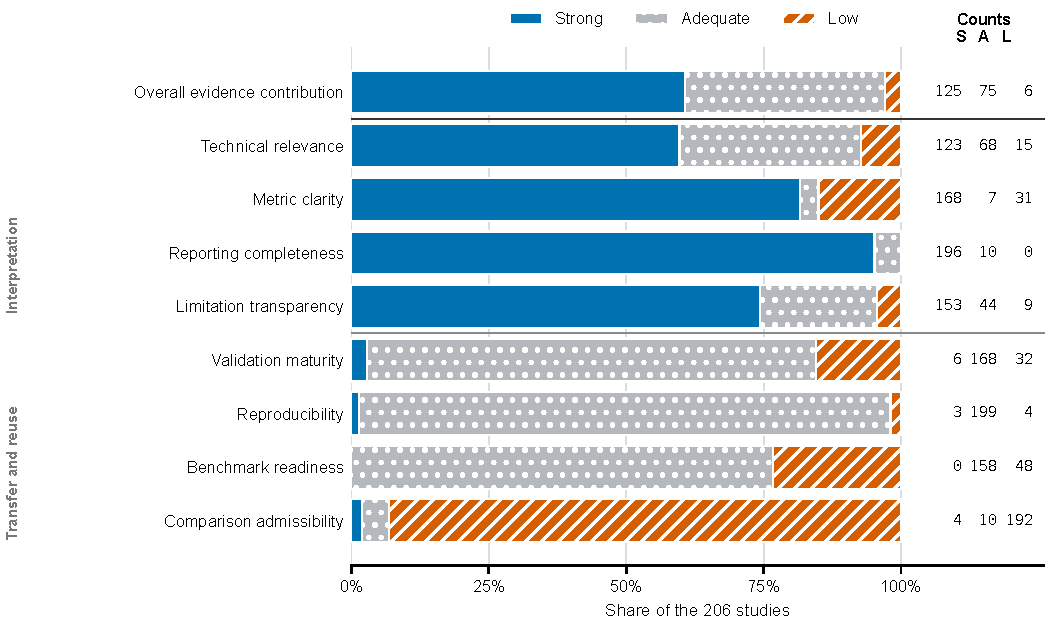
\includegraphics[width=\textwidth]{../manuscript/figures/final_submission_2026-08-25/fig04_tqaf_profile.pdf}
\caption{Full review-specific TQAF profile. The eight dimensions characterize
support for interpretation, transfer, and reuse under the stated scoring
rules. Overall evidence contribution is shown separately; it is not a ninth
appraisal dimension. These descriptive scores do not establish a universal
study ranking.}
\label{fig:s_tqaf_profile}
\end{figure*}

The reproducibility assessment combines parameter reporting with artifact
access: 4 studies were classified as low, 199 as adequate, and 3 as strong.
The benchmark-readiness assessment classified 48 as low, 158 as adequate, and
none as strong. Under these review-specific criteria, strong benchmark
readiness requires an external or common baseline, an open artifact,
admissible outcomes in both functional domains, and strong validation and
reproducibility support within the same evidence chain. These criteria are
more restrictive than either reporting open data or demonstrating a physical
prototype alone.

\begin{figure*}[!t]
\centering
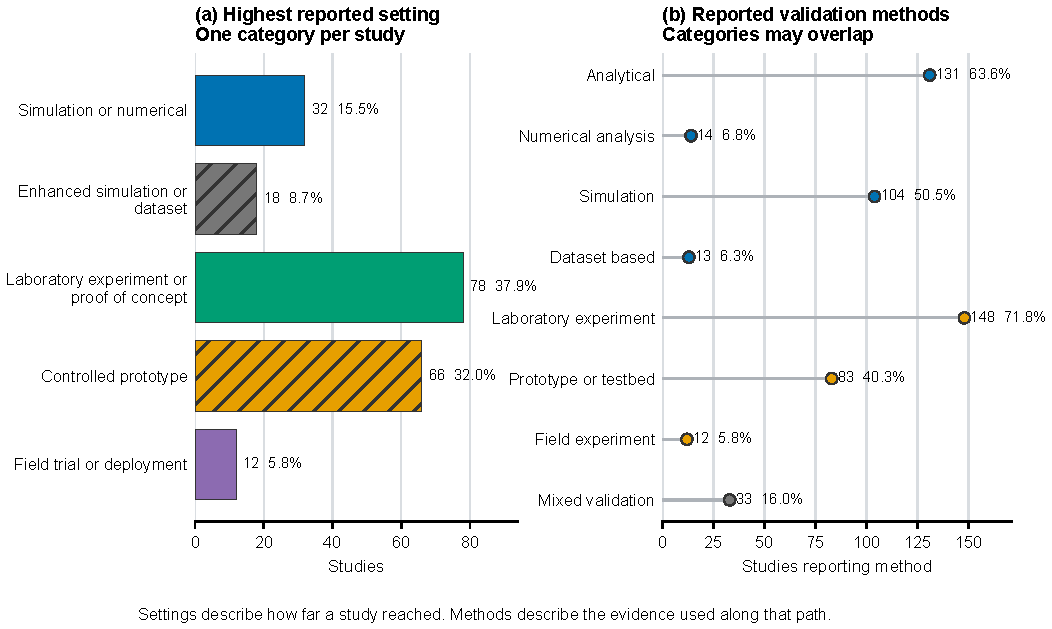
\includegraphics[width=\textwidth]{../manuscript/figures/final_submission_2026-08-25/fig07_validation_profile.pdf}
\caption{Validation settings and overlapping evaluation methods.
Panel (a) assigns each study one highest reported validation setting. Panel
(b) permits overlapping methods: analysis, numerical or dataset-based work,
simulation, laboratory experiments, prototypes, field studies, and mixed
methods may contribute to the same study. Method counts must therefore not
be added to infer a number of independent studies or experimental replications.}
\label{fig:s_validation_methods}
\end{figure*}

The highest-setting classes contain 32 simulation or numerical studies,
18 enhanced-simulation or dataset studies, 78 laboratory or proof-of-concept
studies, 66 controlled prototypes, and 12 field or deployment studies.
Six of the 12 field studies report outcomes in both communication and sensing
at field or deployment level. This study-level classification does not
establish concurrent operation in one configuration or time interval.
S7 preserves separate source locators for the two functions and the available
relationship timing.

\subsection{Technology and 6G Relevance Inventory}

Table~\ref{tab:s_technology_census} preserves the original overlapping
technology counts and the exclusive 6G relevance classification. Technology
labels can occupy different positions in the same signal chain, so their
frequencies do not represent competing architectures or a universal sequence.
For example, photonic integration occurs in 20 studies, distributed acoustic
sensing in 22, machine learning or artificial intelligence in 20, and digital
twins in two. Nineteen studies include specialized mechanisms grouped under
other technology labels. These categories capture device integration,
infrastructure reuse, inference, and additional specialized mechanisms.

\begin{table}[!t]
\caption{Technology-label counts and 6G relevance classes}
\label{tab:s_technology_census}
\centering
\footnotesize
\begin{tabular}{@{}lr@{}}
\toprule
Label & Studies, $n$ \\
\midrule
\multicolumn{2}{@{}l}{\textit{Technology labels: overlapping}} \\
Photonic terahertz generation & 68 \\
Chirped processing & 66 \\
Coherent optics & 64 \\
Multicarrier waveform & 56 \\
Fiber sensing reuse & 22 \\
Photonic integration & 20 \\
Machine learning & 20 \\
Other specialized technologies & 19 \\
Beamforming & 13 \\
Optical phased array & 8 \\
Multiple input multiple output & 7 \\
Digital twin & 2 \\
Optical intelligent surface & 1 \\
\addlinespace[2pt]
\multicolumn{2}{@{}l}{\textit{6G relevance: exclusive}} \\
Direct relevance & 138 \\
Inferential relevance & 64 \\
Weak relevance & 1 \\
Not applicable & 3 \\
\bottomrule
\end{tabular}
\end{table}

Direct 6G relevance means that a report explicitly connects its system to a
6G role; inferential relevance identifies an enabling contribution requiring
additional network context. The remaining classes describe lighter
connections or application settings outside that framing. The application
category ``6G and access'' in Table~\ref{tab:s_application_census} is a separate,
overlapping application label. Neither classification demonstrates a
network-level operating point merely through the presence of a 6G label.

\subsection{Complete Application Inventory}

Table~\ref{tab:s_application_census} preserves all thirteen application
domains and their study counts, conditions, and selected references.
The main article groups these requirements by the experiment needed to test
joint operation; that presentation does not alter the underlying taxonomy.
\begin{table*}[!t]
\caption{Application domains and operating requirements in the reviewed corpus}
\label{tab:s_application_census}
\centering
\footnotesize
\setlength{\tabcolsep}{3pt}
\renewcommand{\arraystretch}{1.05}
\begin{tabularx}{\textwidth}{@{}
>{\raggedright\arraybackslash}p{0.16\textwidth}
>{\raggedright\arraybackslash}p{0.39\textwidth}
>{\raggedright\arraybackslash}X
>{\centering\arraybackslash}p{0.095\textwidth}@{}}
\toprule
\multicolumn{4}{@{}l}{\emph{Network and mobility}} \\
\addlinespace[1pt]
\textbf{Domain, n (\%)} & \textbf{Common communication and sensing role} &
\textbf{Key operating condition} & \textbf{Studies} \\
\midrule
\textbf{6G and access} 100 (48.5\%) & Access and transport with channel, target,
position, or environment sensing & Timing, orchestration, continuity, and
evidence for both functions & \cite{OISAC_SCR00277,OISAC_SCR01049} \\
\addlinespace[1.25pt]
\textbf{Vehicular} 41 (19.9\%) & Vehicle data links with range, motion, pose,
temperature, or channel sensing & Changing geometry, acquisition, tracking, and
service continuity & \cite{OISAC_SCR00123,OISAC_SCR00273} \\
\addlinespace[1.25pt]
\textbf{Optical access} 32 (15.5\%) & Access and transport links with channel,
event, or fiber state sensing & Reach, synchronization, and traffic continuity &
\cite{OISAC_SCR00007,OISAC_SCR01006,OISAC_SCR01049} \\
\addlinespace[1.25pt]
\textbf{Indoor positioning} 13 (6.3\%) & Indoor optical links with user or robot
position and orientation sensing & Geometry, calibration, coverage, and update
continuity &
\cite{OISAC_SCR00910,OISAC_SCR01024} \\
\addlinespace[1.25pt]
\textbf{Data center} 4 (1.9\%) & Short reach data links with channel estimation
or link state sensing & Traffic continuity and calibrated link references &
\cite{OISAC_SCR00007} \\
\bottomrule
\end{tabularx}

\vspace{3pt}
\begin{tabularx}{\textwidth}{@{}
>{\raggedright\arraybackslash}p{0.16\textwidth}
>{\raggedright\arraybackslash}p{0.39\textwidth}
>{\raggedright\arraybackslash}X
>{\centering\arraybackslash}p{0.095\textwidth}@{}}
\toprule
\multicolumn{4}{@{}l}{\emph{Infrastructure}} \\
\addlinespace[1pt]
\textbf{Domain, n (\%)} & \textbf{Common communication and sensing role} &
\textbf{Key operating condition} & \textbf{Studies} \\
\midrule
\textbf{Environmental monitoring} 55 (26.7\%) & Distributed links with vibration,
temperature, or environmental event sensing & Persistent observation,
localization, and traceable reference data &
\cite{OISAC_SCR00957,OISAC_SCR01006,OISAC_SCR01095} \\
\addlinespace[1.25pt]
\textbf{Smart infrastructure} 41 (19.9\%) & Infrastructure links with structural,
motion, or event monitoring & Continuous observation, calibration, and
resilient alert delivery & \cite{OISAC_SCR00277,OISAC_SCR00763,OISAC_SCR01006} \\
\addlinespace[1.25pt]
\textbf{Industrial} 34 (16.5\%) & Industrial data or control with process,
strain, temperature, motion, or position sensing & Delay, continuity,
calibration, and safe operation & \cite{OISAC_SCR00277,OISAC_SCR00376} \\
\addlinespace[1.25pt]
\textbf{Security and surveillance} 26 (12.6\%) & Monitoring links with anomaly,
event, or location sensing & Coverage, event discrimination, and alert latency &
\cite{OISAC_SCR01006} \\
\bottomrule
\end{tabularx}

\vspace{3pt}
\begin{tabularx}{\textwidth}{@{}
>{\raggedright\arraybackslash}p{0.16\textwidth}
>{\raggedright\arraybackslash}p{0.39\textwidth}
>{\raggedright\arraybackslash}X
>{\centering\arraybackslash}p{0.095\textwidth}@{}}
\toprule
\multicolumn{4}{@{}l}{\emph{Human use, extreme settings, and remaining domains}} \\
\addlinespace[1pt]
\textbf{Domain, n (\%)} & \textbf{Common communication and sensing role} &
\textbf{Key operating condition} & \textbf{Studies} \\
\midrule
\textbf{Healthcare} 6 (2.9\%) & Wearable or ambient links with vital sign,
activity, or gesture sensing & Motion robustness, physiological reference,
illumination, and user safety & \cite{OISAC_SCR00001,OISAC_SCR00376} \\
\addlinespace[1.25pt]
\textbf{Aerospace} 20 (9.7\%) & Satellite links with atmospheric or wavefront
sensing & Pointing, turbulence, delay, and link adaptation &
\cite{OISAC_SCR00456} \\
\addlinespace[1.25pt]
\textbf{Underwater} 2 (1.0\%) & Underwater link concepts and subsea data links
with temperature or event sensing & Water attenuation or cable calibration,
packaging, and access & \cite{OISAC_SCR00763,OISAC_SCR01095} \\
\addlinespace[1.25pt]
\textbf{Other} 17 (8.3\%) & Emerging links with range, imaging, object, or
channel sensing & Metrics and reporting specific to the task & \cite{OISAC_SCR00953} \\
\bottomrule
\end{tabularx}
\vspace{1pt}
\parbox{\textwidth}{\raggedright\footnotesize\emph{Note.} Application domains
overlap, so a study may contribute to more than one row. Counts and percentages
describe coverage within the 206 included studies. For each domain, the table
includes a selected study set and lists the corresponding references in the
final column. The 6G and access row identifies the application category, and
the preceding subsection provides the separate 6G relevance classification.\par}
\end{table*}
\subsection{Metric Records Requiring Conservative Interpretation}

The primary metric collection contains 4,779 records, each representing a
reported metric observation rather than an independent study or joint effect.
Within this collection, 118 records are conditional comparison candidates.
Their candidate status does not establish 118 verified cross-study relations,
independent replications, or pooled effects. Compatibility still depends on
the task, quantity, measurement plane, operating conditions, and source-level
evidence, as explained in the main article.

For 92 metric rows, the available source fields supported interpretation in
the original setting with a conservative comparison status. These rows are
retained with their source context; missing comparison information is not
imputed, and their count does not define an effect estimate. S-Evidence and
the metric records preserve the detailed field values and source locators.
Artifact-access classifications combine source reporting with targeted link
checks and describe the documented access route, rather than the completeness
of an independently executed reproduction.

\FloatBarrier
\bibliographystyle{IEEEtran}
\begingroup\small
\bibliography{../manuscript/references_206_candidate,../manuscript/references_companion_21_candidate,../manuscript/references_context_candidate}
\endgroup
\end{document}
